\section{METODOLOGÍA} \label{sec:methodology}

En este capítulo, se describirá la metodología utilizada para conseguir cumplir los objetivos establecidos. 

Se comenzará por discutir el diseño de la investigación y los tipos de variables que serán utilizados a la hora de realizar el estudio. Luego se describirá el enfoque aportado para el preprocesamiento de datos, incluida la limpieza de datos y la selección de características.

Finalmente, se describirán los algoritmos de aprendizaje automático utilizados para el estudio y clasificación de pacientes. 

\subsection{Diseño de Investigación}

Se ha utilizado un enfoque de investigación cuantitativa para examinar la progresión temporal de la bronquiolitis en pacientes pediátricos. Se ha partido de 47 variables descriptivas y de 2 variables que muestran la evolución temporal de los pacientes durante las primeras 24 h de ingreso y que han sido tratadas en el presente trabajo como series temporales. 

\subsubsection{Tipos de Variables}\label{sec:tiposdevariables}

Dentro de las 47 variables descriptivas a utilizar antes mencionadas también se incluyen 4 variables que muestran la evolución temporal por intervalos de los pacientes. Estas variables son:

\begin{itemize}
    \item Flujo de Oxígeno
    \item Frecuencia Respiratoria
    \item Escala SAPI (Sistemas de Alerta Precoz Infantil)
    \item Score Wood-Downes
\end{itemize}

Estas 4 variables no han sido tratadas como series temporales dada la baja frecuencia de recolección durante las primeras 24 h de ingreso; que es el intervalo temporal al que ha sido acotado el estudio. Las tres primeras (Flujo de Oxígeno, Frecuencia Respiratoria y Escala SAPI)variables han sido recopiladas 3 veces durante las primeras 24h del ingreso del paciente pediátrico y la última (Score Wood-Downes) ha sido recogida a la llegada del paciente y a las 24 h. Es decir estas variables describen la estancia del paciente en intervalos.  Estas variables serán catalogadas como \textit{Temporales en Intervalos.} 

Si tratamos estas 3 últimas variables como temporales nos quedarían solamente 36 variables descriptivas. (3 variables temporales $\times$ 3 intervalos + 1 $\times$ 2 intervalos = 11 variables) y por otro lado 2 variables en forma de series temporales. Cada variable de estas contiene 1441 datos. (60 minutos $\times$ 24 horas + 1\textsuperscript{er} dato repetido
= 1441).

Dentro de las 36 variables descriptivas restantes se encuentran 3 variables que dan información más allá de las primeras 24 h de monitorización. Estas variables en principio serán excluidas del estudio y son:

\begin{itemize}
    \item Días con Gafas Nasales
    \item Días con O$_2$
    \item Días con OAF
\end{itemize}

Estas 3 variables serán catalogadas como: \textit{Descriptivas fuera del scope}. El \textit{scope} será básicamente las primeras 24 h de ingreso del paciente pediátrico.

Por último dentro de las 33 variables descriptivas dentro del \textit{scope} se encuentran 2 variables que no son ni cualitativas ni cuantitativas. Estas variables serán catalogadas como \textit{Otras}. Las 31 variables restantes serán catalogadas como \textit{Descriptivas dentro de scope}.

En la tabla \ref{tabla:variables_estudio} se muestran las diferentes variables recopiladas para realizar el presente estudio. 

\begin{table}[H]
    \centering
        \begin{tabular}{| m{5cm} | m{1.75cm} | m{7cm} |}
            \hline Tipo de Variable & Cantidad & Nombres  \\ \hline
            Descriptivas dentro de scope & 31 & Edad, Peso, Sexo, Edad Gestacional (EG), Palivizumab, Lactancia Materna (LM), Dermatitis, Alergias, Tabaco, Enfermedad Base, Radiografía, Analítica, Suero, Etiología, Prematuridad, Alimentación, Sonda Nasogástrica, Gafas Nasales al Ingreso, OAF, OAF al ingreso, OAF tras ingreso, Horas de Ingreso tras inicio OAF, UCIP, Deterioro, Pausas de Apnea, PCT (Procalcitonina en la sangre), PCR (Prueba de Proteína C relativa), Leucocitos, Nautrófilos, Linfocitos y Score Cruces Ingreso  \\ \hline
            Descriptivas fuera de scope & 3 & Días con Gafas Nasales, Días con O$_2$ y Días con OAF. \\ \hline
            Temporales en 3 Intervalos & 11 & Frecuencia Respiratoria (0 - 8 h), Frecuencia Respiratoria (8 - 16 h),
            Frecuencia Respiratoria (16 - 24 h),
            Flujo O$_2$ (0 - 8 h),
            Flujo O$_2$ (8 - 16 h),
            Flujo O$_2$ (16 - 24 h),
            SAPI (0 - 8 h),
            SAPI (8 - 16 h), 
            SAPI (16 - 24 h), Score Wood-Downes Ingreso y Score Wood-Downes 24 h . \\ \hline
            Series Temporales & 2 & Frecuencia Cardiaca, Saturación de Oxígeno \\ \hline
            Otras & 2 & Notas e Identificador Paciente. \\ \hline
        \end{tabular}
    \caption{Variables Usadas en el Estudio}\label{tabla:variables_estudio}
\end{table}

Las variables temporales han sido recopiladas durante las primeras 24 h del ingreso del paciente pediátrico cuando mostraba un cuadro bronquiolítico. La frecuencia con la que han sido recopilados los datos ha sido de 1 vez cada minuto. En la siguiente figura \ref{fig:fc-JJB} se muestra un ejemplo de la evolución  variable \textit{Frecuencia Cardiaca} en forma de serie temporal y de la misma forma la figura \ref{fig:satO2-JJB} pero para la \textit{Saturación de O$_2$}. Estas dos series temorales pertenecen a la evolución del paciente pediátrico \textit{JJB\_11182744}.

\begin{figure}[H]
    \centering
    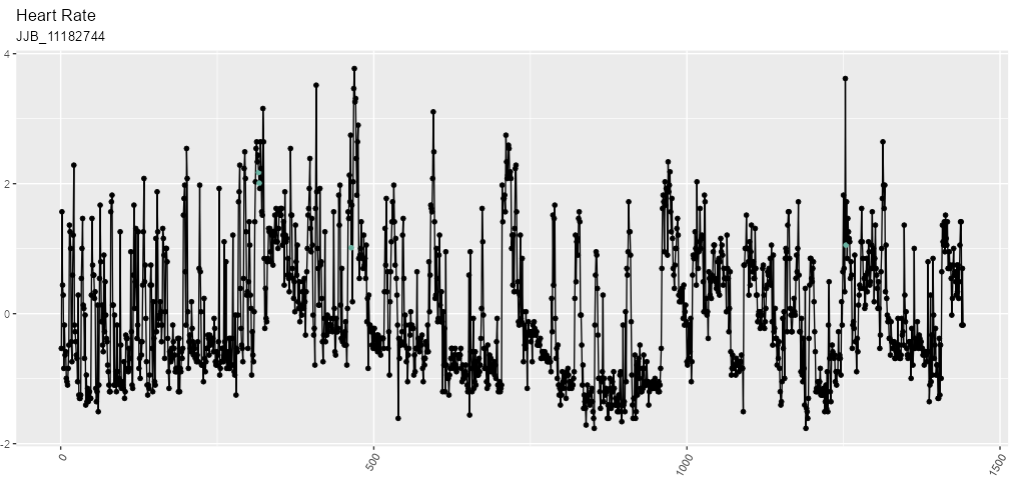
\includegraphics[scale=0.70]{./img/Heart-Rate-JJB.png}
    \caption{Valores de Frecuencia Cardíaca del paciente \textit{JJB\_11182744}}
    \label{fig:fc-JJB}
\end{figure}

\begin{figure}[H]
    \centering
    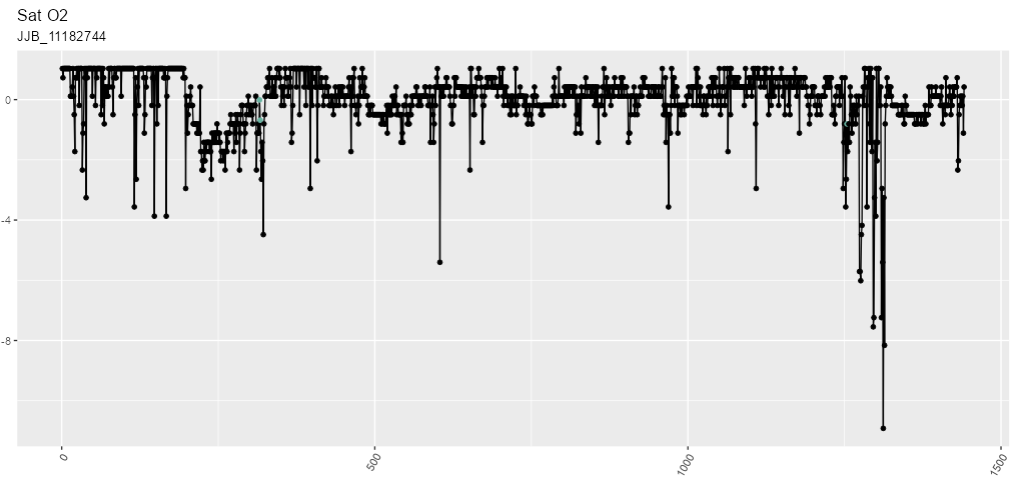
\includegraphics[scale=0.70]{./img/SatO2-JJB.png}
    \caption{Valores de Saturación de O$_2$ del paciente \textit{JJB\_11182744}}
    \label{fig:satO2-JJB}
\end{figure}

A la hora de trabajar con variables temporales se ha de tener en cuenta que los datos temporales pueden ser de dos tipos: \textit{Discretos} o \textit{Continuos}. Los datos discretos son aquellos que se recogen en intervalos de tiempo, por ejemplo, el número de pacientes que llegan a un hospital cada hora. Los datos continuos son aquellos que se recogen de forma continua, por ejemplo, en nuestro caso la saturación y frecuencia cardíaca de un paciente cada minuto.

Para terminar este punto \ref{sec:tiposdevariables} una última cuestión a valorar son las variables cualitativas y cuantitativas que se han recopilado. Las variables cualitativas son aquellas que describen una cualidad del paciente, por ejemplo, el sexo o la edad gestacional. Las variables cuantitativas son aquellas que describen una cantidad del paciente, por ejemplo, la frecuencia cardíaca o la saturación de oxígeno.

En la siguiente tabla \ref{tabla:cuali_cuanti} se muestra la división entre variables cualitativas y cuantitivas recopiladas en el estudio y dentro del \textit{scope}.

\begin{table}[H]
    \centering
        \begin{tabular}{| m{5cm} | m{1.75cm} | m{7cm} |}
            \hline Tipo de Variable & Cantidad & Nombres  \\ \hline
            Cuantitativas & 15 & Edad, Peso, Edad Gestacional (EG), Horas de Ingreso tras inicio OAF, PCT (Procalcitonina en la sangre), PCR (Prueba de Proteína C relativa), Leucocitos, Nautrófilos, Linfocitos, Frecuencia Respiratoria (0 - 8 h), Frecuencia Respiratoria (8 - 16 h),
            Frecuencia Respiratoria (16 - 24 h),
            Flujo O$_2$ (0 - 8 h),
            Flujo O$_2$ (8 - 16 h),
            Flujo O$_2$ (16 - 24 h). \\ \hline
            Cualitativas & 27 & Sexo, Palivizumab, Lactancia Materna (LM), Dermatitis, Alergias, Tabaco, Enfermedad Base, Radiografía, Analítica, Suero, Etiología, Prematuridad, Alimentación, Sonda Nasogástrica, Gafas Nasales al Ingreso, OAF, OAF al ingreso, OAF tras ingreso, UCIP, Deterioro, Pausas de Apnea, Score Cruces Ingreso, SAPI (0 - 8 h),
            SAPI (8 - 16 h), 
            SAPI (16 - 24 h), Score Wood-Downes Ingreso y Score Wood-Downes 24 h. \\ \hline
            Otras & 2 & Notas e Identificador Paciente. \\ \hline
        \end{tabular}
    \caption{Variables Cualitativas y Cuantitativas Dentro del \textit{Scope}}\label{tabla:cuali_cuanti}
\end{table}

\subsection{Procesamiento de los Datos}

En este apartado se describirá el procesamiento de los datos realizado para el presente estudio.

\subsubsection{Limpieza de Datos}

En primer lugar se ha realizado una limpieza de datos. Esta limpieza de datos ha consistido en varios pasos: 

\begin{enumerate}
    \item \textbf{Contraste de Archivos:} Contrastar que los diferentes archivos de datos no contenían datos duplicados o incoherencias.
    \item \textbf{Cálculo de Medias:} Calcular de manera automatizada las medias de \textit{Frecuencia Respiratoria} y \textit{Saturación de Oxígeno} cada hora.
    \item \textbf{Datos Faltantes:} Determinar que pacientes y variables tenían un alto número de datos faltantes y eliminarlos del estudio.
    \item \textbf{Variables No Relevantes:} Eliminar variables que no aportaban información relevante para el estudio.
\end{enumerate}

 \paragraph*{Contraste de Archivos}

Por parte del hospital se han recopilado 2 archivos de datos diferentes. Estos archivos de datos son:

\begin{itemize}
    \item \textbf{Archivo de Datos de Pacientes:} Este archivo contiene información descriptiva de los pacientes pediátricos. En este archivo se encuentran las variables contenidas en la tabla \ref{tabla:cuali_cuanti}. Este archivo contiene 47 variables y 79 pacientes.
    \item \textbf{Carpeta de Datos de Monitorización:} En esta carpeta se almacena un archivo por paciente. Cada archivo contiene información temporal de los pacientes pediátricos. En este archivo se encuentran las variables \textit{Series Temporales} en la tabla \ref{tabla:variables_estudio}. Por cada archivo se tienen 2 variables temporales (Saturación de O$_2$ y Frecuencia Cardiaca) y 1441 datos por paciente.
\end{itemize}

La Carpeta de Datos de Monitorización contiene 79 archivos de datos y el Archivo de Datos de Pacientes contiene 79 pacientes. Por lo tanto, se ha de contrastar que los datos de los pacientes contenidos en el Archivo de Datos de Pacientes estén contenidos en la Carpeta de Datos de Monitorización o si existen pacientes duplicados.

La cabecera de la Carpeta de Datos de Monitorización es la siguiente:
\begin{figure}[H]
    \centering
    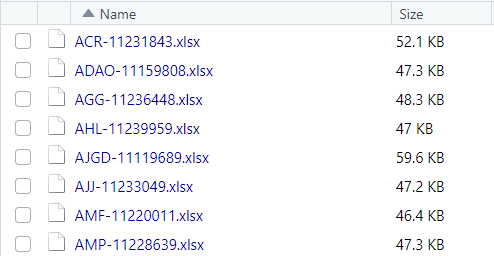
\includegraphics[scale=0.70]{./img/Carpeta-Monitor.png}
    \caption{Cabecera de la Carpeta de Datos de Monitorización}
    \label{fig:cabecera_monitorizacion}
\end{figure}

Y las primeras columnas del Archivo de Datos de Pacientes son las siguientes:
\begin{figure}[H]
    \centering
    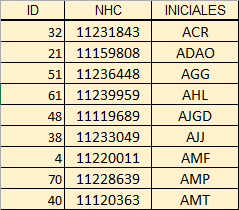
\includegraphics[scale=1.0]{./img/Archivo-Monitor.png}
    \caption{Cabecera de la Carpeta de Datos de Monitorización}
    \label{fig:cabecera_monitorizacion}
\end{figure}

Este contraste se ha automatizado de manera que para futuros estudios se pueda realizar de manera rápida y eficiente. El resultado de este contraste ha sido que los datos de los pacientes contenidos en el Archivo de Datos de Pacientes están contenidos en la Carpeta de Datos de Monitorización. Existían algunas desviaciones en los nombres pero fuero corregidas. Por lo tanto, no existen pacientes duplicados y se puede continuar con el estudio.

\paragraph*{Cálculo de Medias}

En el Archivo de Datos de Pacientes venían calculadas las medias de \textit{Frecuencia Respiratoria} y \textit{Flujo de Oxígeno} cada hora. Estas medias han sido re-calculadas de manera automatizada para cada paciente y se han añadido al Archivo de Datos de Pacientes. Además de estas 2 medias se han hecho dos trasformaciones en los datos de \textit{Frecuencia Cardiaca} que se explicarán más tarde y se han calculado sus respectivas medias por hora. 

Se han calculado dos tipos de medias: 

\begin{itemize}
    \item \textbf{Medias No Nulas:} Se han calculado las medias de aquellos intervalos de hora dentro de las 24 h que no presentaban valores faltantes.
    \item \textbf{Medias Nulas:} Se han calculado las medias de aquellos intervalos de hora dentro de las 24 h sin importar si había momentos de valores valores faltantes dentro del intervalo hora.
\end{itemize}

El resultado para el paciente \textit{JJB\_11182744} ha sido el siguiente mostrado en la Tabla \ref{tabla:medias-JJB}:

% Se comienza una página nueva sin formato (sin número de página y sin encabezado/pie de página):
\newpage
\thispagestyle{empty}

% Se modifica la geometría (los márgenes) de la página y se coloca en formato horizontal:
\newgeometry{top=10mm, bottom=10mm, left=12mm, right=12mm}
\begin{landscape}

    \begin{table}[!ht]
        \centering
        \begin{tabular}{|l|l|l|l|l|l|l|l|l|l|l|l|}
        \hline
            hour & n & Missing\_FC & Missing\_SO2 & Mean\_FC & Mean\_SO2 & Mean\_Q & Mean\_SC & Mean\_FC\_NA & Mean\_SO2\_NA & Mean\_Q\_NA & Mean\_SC\_NA \\ \hline
            18 & 43 & 0 & 0 & 140,4186047 & 98,23255814 & 0,552067823 & -0,205230874 & 140,4186047 & 98,23255814 & 0,552067823 & -0,205230874 \\ \hline
            19 & 60 & 0 & 0 & 137,4666667 & 99,1 & 0,500688619 & -0,356544211 & 137,4666667 & 99,1 & 0,500688619 & -0,356544211 \\ \hline
            20 & 60 & 0 & 0 & 143,0166667 & 98,46666667 & 0,613802318 & -0,07205686 & 143,0166667 & 98,46666667 & 0,613802318 & -0,07205686 \\ \hline
            21 & 60 & 0 & 0 & 141,7 & 97,13333333 & 0,567600299 & -0,139547853 & 141,7 & 97,13333333 & 0,567600299 & -0,139547853 \\ \hline
            22 & 60 & 0 & 0 & 135,3666667 & 92,11666667 & 0,479248047 & -0,464188074 & 135,3666667 & 92,11666667 & 0,479248047 & -0,464188074 \\ \hline
            23 & 60 & 2 & 2 & ~ & ~ & ~ & ~ & 164,3448276 & 95,12068966 & 0,867006799 & 1,021202963 \\ \hline
            00 & 60 & 0 & 0 & 162,0666667 & 98,5 & 0,918496135 & 0,904426753 & 162,0666667 & 98,5 & 0,918496135 & 0,904426753 \\ \hline
            01 & 60 & 0 & 0 & 150,9833333 & 97,13333333 & 0,729509118 & 0,336306366 & 150,9833333 & 97,13333333 & 0,729509118 & 0,336306366 \\ \hline
            02 & 60 & 1 & 0 & ~ & 95,98333333 & ~ & ~ & 155,559322 & 95,98333333 & 0,762103523 & 0,570866889 \\ \hline
            03 & 60 & 0 & 0 & 142,3166667 & 96,01666667 & 0,606131522 & -0,107938147 & 142,3166667 & 96,01666667 & 0,606131522 & -0,107938147 \\ \hline
            04 & 60 & 0 & 0 & 142,2166667 & 96,86666667 & 0,569912026 & -0,113064045 & 142,2166667 & 96,86666667 & 0,569912026 & -0,113064045 \\ \hline
            05 & 60 & 0 & 0 & 130,6166667 & 97,8 & 0,37096502 & -0,70766824 & 130,6166667 & 97,8 & 0,37096502 & -0,70766824 \\ \hline
            06 & 60 & 0 & 0 & 155,8166667 & 96,4 & 0,762258703 & 0,584058113 & 155,8166667 & 96,4 & 0,762258703 & 0,584058113 \\ \hline
            07 & 60 & 0 & 0 & 132,55 & 96,73333333 & 0,405018753 & -0,608567541 & 132,55 & 96,73333333 & 0,405018753 & -0,608567541 \\ \hline
            08 & 60 & 0 & 0 & 129,4833333 & 97,06666667 & 0,344631214 & -0,765761753 & 129,4833333 & 97,06666667 & 0,344631214 & -0,765761753 \\ \hline
            09 & 60 & 0 & 0 & 127,8166667 & 97,18333333 & 0,312055141 & -0,85119339 & 127,8166667 & 97,18333333 & 0,312055141 & -0,85119339 \\ \hline
            10 & 60 & 0 & 0 & 151,2166667 & 96,43333333 & 0,703296936 & 0,348266795 & 151,2166667 & 96,43333333 & 0,703296936 & 0,348266795 \\ \hline
            11 & 60 & 0 & 0 & 156,55 & 97,41666667 & 0,87619425 & 0,621648034 & 156,55 & 97,41666667 & 0,87619425 & 0,621648034 \\ \hline
            12 & 60 & 0 & 0 & 145,95 & 98,1 & 0,685284072 & 0,078302822 & 145,95 & 98,1 & 0,685284072 & 0,078302822 \\ \hline
            13 & 60 & 0 & 0 & 146,4166667 & 98,13333333 & 0,704465169 & 0,10222368 & 146,4166667 & 98,13333333 & 0,704465169 & 0,10222368 \\ \hline
            14 & 60 & 0 & 0 & 129,9333333 & 97,08333333 & 0,372386073 & -0,742695211 & 129,9333333 & 97,08333333 & 0,372386073 & -0,742695211 \\ \hline
            15 & 60 & 1 & 1 & ~ & ~ & ~ & ~ & 155,220339 & 92,6779661 & 0,833584194 & 0,553490963 \\ \hline
            16 & 60 & 0 & 0 & 143,6333333 & 93,95 & 0,628285376 & -0,040447154 & 143,6333333 & 93,95 & 0,628285376 & -0,040447154 \\ \hline
            17 & 60 & 0 & 0 & 141,8666667 & 96,01666667 & 0,596238571 & -0,131004689 & 141,8666667 & 96,01666667 & 0,596238571 & -0,131004689 \\ \hline
            18\_1 & 18 & 0 & 0 & 156,1111111 & 96,05555556 & 0,890367072 & 0,599151036 & 156,1111111 & 96,05555556 & 0,890367072 & 0,599151036 \\ \hline
        \end{tabular}
        \caption{Medias Nulas y No Nulas de \textit{Frecuencia Cardíaca}, \textit{Saturación de O$_2$}, \textit{Cuantiles Cardíacos} y \textit{Frecuencia Cardíaca Escalada}  por hora para el paciente \textit{JJB\_11182744}}\label{tabla:medias-JJB}
    \end{table}

% Se devuelve el formato y la geometría de la página a sus valores originales:
\end{landscape}
\restoregeometry 

\paragraph*{Datos Faltantes}

Se ha realizado un estudio de los datos faltantes en el estudio. Este estudio ha consistido en determinar que pacientes y que variables tenían un alto número de datos faltantes y eliminarlos del estudio. 


